\documentclass{l4proj}
%% Language and font encodings
\usepackage[english]{babel}
\usepackage[utf8x]{inputenc}
\usepackage[T1]{fontenc}
\usepackage[colorinlistoftodos]{todonotes}
\usepackage[colorlinks=true, allcolors=blue]{hyperref}
\usepackage{listings}
\usepackage[newfloat]{minted}
\usemintedstyle{emacs}
\usepackage{pgfplots}
\pgfplotsset{compat=1.8}
\usepackage{filecontents}
\usepackage{graphicx}
\usepackage{adjustbox}
\usepackage{tikz}
\usepackage{enumerate}
\usepackage{enumitem}
\usepackage{url}
\usepackage{amssymb}
\usepackage{amsmath}
\usepackage{caption}
\usepackage{subcaption}
\usepackage{inconsolata}
\newcommand{\code}[1]{\texttt{#1}}
\newenvironment{codelisting}{\captionsetup{type=listing}}{}
\SetupFloatingEnvironment{listing}{name=Code Sample}
\begin{filecontents*}{data.csv}
name map length time
allterms 	0.4554	358.5  	2.51435
ne 			0.3979  93.45  	0.4132
tfidf 		0.3038  10  	0.13675
subject 	0.184  	9.75  	0.1578
\end{filecontents*}

\title{Public vs. Private: \newline Identifying Public Domain Knowledge}
\author{Kelvin Fowler\\2083905f}
\date{\today}

\begin{document}
\maketitle

\begin{abstract}
The current system of sensitivity review used in the archival process of government documents cannot keep up with the rapid creation of new content. The process is also cumbersome and insecure.
Information Retrieval techniques can be leveraged to vastly improve this operation. This project provides a prototype of a system and an interface, incorporating these information retrieval techniques, to allow archivists to identify information from documents which already exist within the public domain. Evaluation deemed the prototype to be fairly successful, however various shortcomings were discovered, which could be addressed in future work.
\end{abstract}

\renewcommand{\abstractname}{Acknowledgements}
\begin{abstract}
I would like to thank my supervisors, Dr. Craig Macdonald and Graham McDonald, for their continued guidance throughout the course of this project.
\end{abstract}

\educationalconsent
\tableofcontents

% MAX 2 PAGES
\chapter{Introduction}
\pagenumbering{arabic}

\section{Aims}
This project aims to deliver a prototype of a system which can be used to assist the process of identifying public domain knowledge within potentially sensitive government documents. The project will use information retrieval (IR) techniques to present public domain documents which could help archivists to make an informed choice during sensitivity review. An archivist then can compare information in government documents to information in the public domain in order to ensure no new information is being inadvertently released.

The public domain is defined as that information which is available to the public, without legal restrictions, such as news articles.

\section{Motivations}
Document review within government archives faces major problems today. There is a constant barrage of new documents which must be archived and eventually reviewed, driven by the rapid creation of new artefacts through technology. Each email and memo is now automatically saved and must, at some point, be reviewed.

Further to this, the current system of document review involves no integrated public domain knowledge checking process. Often the substitute for this is a simple web search, which poses many security risks. The search terms themselves could be very sensitive and yet they are being exposed to the internet, and as such, are vulnerable to unintended discovery.

Understanding this, the final product should be a system which can keep up with the vast number of documents which need to be reviewed within archives. A system which is encapsulated and secure when it comes to further research on the content of a document is also sought.

Interestingly, this field has experienced some media coverage in recent times, with certain current affairs being directly linked to sensitive documents. In the case of the Hillary Clinton email scandal, the FBI used technology to aid their process in reviewing these emails for sensitivities~\cite{cnnclinton}. 

Combining these concerns this project strives to produce a highly practical and helpful system, which can inspire and encourage further work into this problem domain. To understand further motivations and context behind this project, see Chapter \ref{relatedliterature}.

\section{Terminology}
Throughout this document certain terms will be used which may not be familiar.
A \textbf{Source Document} is the document which is being reviewed. It is the document from which queries are generated for IR.
A \textbf{Target Document} is a document in the public domain which may contain information relevant to the review of a source document. These are the documents are which are to be retrieved.

\section{Structure}
This dissertation will take the following structure.
Chapter \ref{relatedliterature} investigates the project's relevance through review of some related literature.
Next, the planning, requirements and design of the system are discussed in Chapter \ref{requirementsanddesign}.
Chapters \ref{serverimplementation} and \ref{clientimplementation} detail the implementation challenges of the system's components.
Chapter \ref{evaluation} explains the experimentation and evaluation undertaken to determine the systems effectiveness. The dissertation concludes with learnings and potential future work in Chapter \ref{conclusion}.

% MAX 2 PAGES
\chapter{Related Literature} \label{relatedliterature}
The Freedom of Information Act (2000) allows for all documents held by government to be accessed by the public, upon request, with certain exemptions~\cite{foi}. These exemptions could be negative sentiment towards another country or the identity of confidential informants, or any other specific sensitivity. With these exemptions in mind, government must decide if any given document can be released to the public.
The current sensitivity review procedures used by government archivists are less then ideal. Paper documents must be read in full and much interdepartmental conversation must take place before a decision regarding sensitivity can be made. Digital records, of which there are constantly increasing numbers, only make this process even more complicated. This explosion in magnitude poses many potential problems for archiving organisations, such as ``What to Keep?'' and how to effectively identify sensitivities~\cite{moss2012have}. The current process is unreasonable and impractical in today's digital context~\cite{allan2014record}.

\section{Sensitivity Review}
Some work has already been done to begin to tackle this issue of digital sensitivity review. Prior to review a ``classifier'' may be used to automatically identify potential sensitivities through use of named entities and document sentiment~\cite{mcdonald2014towards}. This type of work can be used to lower the burden on reviewers by attempting to identify documents which may be of the most concern.

In other research into the challenges and potential avenues for improving the digital sensitivity review process it was found that document reviewers are reluctant to trust technology alone to identify sensitivities, and that a manual review process will likely always be necessary~\cite{gollins2014using}. 
As such, technology which can assist the manual review process (such as that developed in this project) will be increasingly important as the review process is improved and iterated upon.

Sensitivity review is a category of Technology Assisted Review, a field which aims to provide solutions to document review problems using technology. Another, very successful, application of Technology Assisted Review is E-Discovery. This is the discovery of all relevant documents pertaining to the opposing party in a civil litigation case. The idea being that each party should have access to all documents that they are legally entitled to view, so as to gain any possible advantage. Information retrieval has been used extensively to provide E-Discovery services, and is an extremely successful and high profile application of this technology~\cite{oard2013information}. E-Discovery is a high recall task, which means it focusses on returning all of the relevant documents rather than returning the most relevant ones. At a high-level, sensitivity review is also a high recall task, in that all sensitive documents must be found. In the case of this project, however, identifying public domain knowledge is a high precision task. Only one relevant target document is needed to identify the contents of a source document as existing in the public domain.
\section{Information Retrieval}
The intended final product of this project acts as a highly focussed automatic search engine for public domain documents. To facilitate this, some underlying search engine must be in place to process queries and return results. This is done through a search engine specifically designed for this type of information retrieval. Two such search engines are Terrier and Lucene~\cite{macdonald2012puppy, terrier, lucene}. These search engines are capable of performing many different tasks outside of the realm of this project, but are configurable to each specific use case. This type of technology is also used extensively in the works discussed above.

Further to searching, it is important to link the information in a target document to the public domain in some way.
There has been some work into automatically identifying key named entities and concepts witthin documents. One such work is Wikify~\cite{Mihalcea:2007:WLD:1321440.1321475}. Wikify automatically hyperlinks phrases and entities to their relevant Wikipedia articles~\cite{wikipedia}. A system which can understand and identify the best and most important entities within a document is extremely useful in the context of this project, where some kind of searching based on the content of a given source document is a key aim.

This project differs somewhat from the standard search task familiar to most people, that of a free-form query entered by the user, as exemplified by Google~\cite{google}. This type of searching is known as Ad-Hoc Retrieval~\cite{baeza1999modern}. The queries formed in this project are, instead, formulated as subsets of the collection of terms a source document.
\section{The Need for this Project} \label{needs}
In recent times, a great deal more files have been generated by government than ever before. E-mail and digital documents are automatically archived and all must be reviewed and released to the public as mandated by law.
This project seeks to address and help remedy some of these issues by providing efficient and effective tools to ease the digital transition.
These needs are summarised below:
\begin{enumerate}[label=\textbf{Need.\arabic*}]
\item Efficient and effective tool to review digital documents.
\item An easier and better way to review public domain knowledge in the context of a source document.
\item Encapsulated environment to do sensitive public domain research.
\end{enumerate}

% MAX 5 PAGES
\chapter{Requirements and Design} \label{requirementsanddesign}
Before beginning implementation, some initial planning was performed to understand the key requirements of the system. This chapter outlines these requirements as well as those requirements that materialized through the course of the project. Further to this, the architecture and technologies used in the project are introduced.
\section{Requirements}
Initially the project's requirements were elicited from the project supervisors, who have extensive knowledge of the problem domain, through related research and a working relationship with the The National Archives of the UK and Scotland.
These initial requirements allowed the developer to begin implementation, after which more detailed requirements were identified through discussion and experimentation. The progress and requirements were reviewed at weekly meetings, however the process of implementation was fairly fluid, allowing for experimentation and changing priorities. This loosely follows an agile approach, however it is not particularly important to label the process so specifically~\cite{Sommerville:2010:SE:1841764}.

\subsection{Functional Requirements}
These functional requirements were compiled throughout the course of the project and evolved as features were experimented with.
The functional requirements of the project were categorised using the MoSCoW method (\textbf{Must Have}, \textbf{Should Have}, \textbf{Could Have} or \textbf{Would Like to Have})~\cite{storer_lecture_2014}. These were further ratified through user stories, which means summarising the requirement through a user scenario using the template ``\textit{As a..., I want to..., So that}"~\cite{storer_lecture_2014}. User stories help us to understand why a requirement is necessary and how it benefits the end user. Further to this a more detailed use case to contextualize the following requirements can be given:\\ 
\textit{``Bob is an archivist at the national archives. He must review a collection of emails for sensitivities. Using the new tool he loads up the collection of the emails. When he opens the first email, some relevant news articles are automatically retrieved at the same time. He reads some of the source document and also the top news article. This news article confirms that the content of the email is already in the public domain. Bob classifies the email as not sensitive and opens the next email to repeat the process.''}
\paragraph{Must Have}
These are the requirements the the project must fulfil to be considered successful.
\begin{enumerate}[label=\textbf{M.\arabic*}]
\item Allow user to identify when a document contains public domain knowledge. \\
\textit{As a} document reviewer, \\
\textit{I want} the ability to decide that a document contains public domain knowledge \\
\textit{So that} I can make a decision regarding its status. \\
\item Frontend user interface displaying source document for review and target documents automatically identified by the software. \\
\textit{As a} document reviewer, \\
\textit{I want} to view both the document up for review and associated public domain documents \\
\textit{So that} I can easily compare the contents of both and see what is known in the public domain.
\item Trials of different retrieval methods and some form of quantitative analysis based on these. \\
\textit{As a} document reviewer, \\
\textit{I want} to be confident that this software will return the most relevant results in reasonable time, \\
\textit{So that} I can trust the service to return excellent related documents.
\end{enumerate}
\paragraph{Should Have}
These are the requirements which are not vital but are to be fulfilled if possible.
\begin{enumerate}[label=\textbf{S.\arabic*}]
\item Generate suggested queries to allow user to refine returned related documents. \\
\textit{As a} document reviewer, \\
\textit{I want} to refine search terms for related documents, \\
\textit{So that} more relevant documents are returned.
\item Ability to run custom queries. \\
\textit{As a} document reviewer, \\
\textit{I want} to write my own queries, \\
\textit{So that} I can retrieve the refine my queries for better results.
\item Date range searches. \\
\textit{As a} document reviewer, \\
\textit{I want} to limit date range for retrieval of related documents, \\
\textit{So that} I can ensure relevance of related documents.
\end{enumerate}
\paragraph{Could Have}
These requirements should only be implemented if all of the above requirements have been completed.
\begin{enumerate}[label=\textbf{C.\arabic*}]
\item Machine learning to improve system performance over time based on usage by reviewers. \\
\textit{As a} document reviewer, \\
\textit{I want} my actions using the system to improve its performance to better suit my needs, \\
\textit{So that} it is easier to find related documents that I would deem relevant.
% \item Tf-idf (Term Frequency - Inverse Document Frequency) analysis to better identify relevant documents. \\
% \textit{As a} document reviewer, \\
% \textit{I want} to only have returned to me related documents which have been identified as containing search terms in meaningful ways, \\
% \textit{So that} I can be sure the returned documents contain information as relevant as possible to the search terms.
\end{enumerate}
\paragraph{Would Like To Have}
These are requirements which are outside the scope of this project and are not deemed important enough to be implemented within the current time frame.
\begin{enumerate}[label=\textbf{W.\arabic*}]
\item Wikify! Like functionality to automatically highlight and link to concepts in source documents which have Wikipedia articles associated with them. \\
\textit{As a} document reviewer, \\
\textit{I want} to have easy access to Wikipedia articles of items mentioned in the document I am reviewing, \\
\textit{So that} I can easily find out more about concepts mentioned in documents.
\item Eye tracking to automatically identify points of interest in the source document from which to formulate queries. \\
\textit{As a} document reviewer, \\
\textit{I want} the system to react to what my eyes are drawn to, \\
\textit{So that} retrieved target documents are dictated by my actions.
\end{enumerate}
\subsection{Non-Functional Requirements}
Non-Functional requirements are those requirements that do not define the specific behaviour of the system, but rather how the system performs.
\begin{enumerate}[label=\textbf{NF.\arabic*}]
\item Intuitive user interface.
\item Results must be relevant.
\item Must return results in reasonable time.
\item Scalability to handle large amounts of files.
\item Robust and fault tolerant.
\end{enumerate}

\section{Design and Architecture}
The application is based on a client-server design. More specifically, a web application acts as a client which interfaces with a RESTful API acting as a server. This paradigm was chosen so as to abstract all of the complicated logic away from the system presented to the user. This also meant that implementation could be split across the two distinct components, simplifying development.
The client communicates with the server using HTTP requests which request information from the server or update information on the server. An overview of the system can be seen in Figure~\ref{architecture} with details following in the sections below.
\begin{figure}[H]
\centering
\includegraphics[scale=0.45]{images/BigBox}
\caption{Overview of System Architecture}
\label{architecture}
\end{figure}

\subsection{Server Architecture}
\paragraph{Information Retrieval}
The project depends on some IR system so that the Must Have requirements can be fulfilled (specifically, \textbf{M.3}). The IR system chosen for these needs was Terrier. Terrier is a open-source search engine with an extensive Java API allowing it to be easily used for development of various IR tasks~\cite{terrier, macdonald2012puppy}.
Terrier, being developed at The University of Glasgow, was the best and obvious choice of IR technology for the project. The local expertise meant that problems encountered could be easily resolved or explained, ensuring minimal downtime due to learning.
Other choices could have been Apache Lucene or MG4J~\cite{middleton2007comparison}.
\paragraph{Programming Language}
As Terrier had already been chosen as the IR tool for the project, it was necessary that the supporting system was written in Java, in order that it could interact with the Terrier Java API.

\paragraph{Persistence}
One fundamental aspect of Terrier is the concept of indexes. These are files containing the important information from a collection of documents necessary for information retrieval. This provides a persistent data storage mechanism which can be used to store additional information about documents or groups of documents. This kind of data is saved in a \textit{meta-index} within a normal index.

Terrier is able to handle TREC test collections, which allow documents to be defined through tags, much like XML \cite{trecnist}.
Since Terrier is easily configurable to a custom version of this TREC document style it was decided that the documents pertinent to the project should be arranged like this.
This provides an opportunity to store additional information within new tags in each \code{.trec} document. This technique is used to save information too large for the Terrier meta-index.
These techniques produce a fully functional state system capable of retaining all the necessary information needed for the system.

This design entirely eliminates the need for a DBMS (Database Management System) like PostgreSQL and the complicated Java Object to Database Model mapping that often comes with such designs.

\paragraph{Natural Language Processing (NLP)}
As Terrier mandated the use of Java, any NLP framework chosen was required to have a Java API.
Stanford Natural Language Processing was used as an NLP framework to identify terms from which to form effective queries~\cite{manning-EtAl:2014:P14-5}. The Java API allows text to be analysed and annotated. More specifically, the named entity identification capability of StandordNLP was used~\cite{finkel2005incorporating}.
Stanford NLP was initially chosen due to its preferable documentation. It also offers the ability to identify specifically which tokenisers to use when processing some text, allowing the developer to streamline the NLP process to their specific use-case.

\paragraph{RESTful API}
Jersey is a framework which provides a reference implementation of the JAX-RS API as defined by Oracle, allowing a REST API to be developed~\cite{jersey,jaxrsapi}.
Jackson is used alongside Jersey to provide support for JSON~\cite{jackson}. This allows the frontend and backend to communicate using one format. It handles the conversion of JSON to Java Objects and vice versa.
This set-up allows one to define a fully functional HTTP REST API which can consume and produce JSON.

\subsection{Client Architecture}
The web application maintains no state between usages, but rather requests all necessary data from the server upon loading. Having no state system in the client application greatly reduces the complexity of the web application.
\paragraph{Model View ViewModel}
The architecture of the frontend user interface is based around the Model View ViewModel (MVVM) design pattern. Facilitated by the JavaScript library Knockout.js, MVVM allows us to consolidate the logic associated with the DOM (Domain Object Model) into one place~\cite{knockout}.
This vastly simplifies the automatic update of DOM elements based on JS variables.
This lends itself well to the problem domain of many rapidly changing documents and results sets as the user identifies relevant documents.

There are various other libraries that allow for similar designs, however developer familiarity with Knockout's syntax and best practices meant that development was easy and fast.
This was important as the learning curve for the backend technologies required more attention.

\paragraph{Style}
Although our data manipulation is handled by Knockout, information must also be presented in an intuitive and user friendly way. There are many frameworks which provide pre-built components to build user interfaces but Bootstrap was chosen mainly due to familiarity reasons. It provides myriad customisable components, as well as being extremely well documented~\cite{bootstrap}. This dramatically simplifies the rapid development of a user interface.

\paragraph{AJAX}
JQuery is used in the frontend to interface with the backend through HTTP (AJAX) requests~\cite{jquery}. JQuery provides a very well documented and widely adopted API for this. JQuery is a dependency of both Knockout and Bootstrap and so utilizing its already present features was sensible and easy.

\paragraph{Web Application Framework}
The web application currently uses an Express.js server running on Node.js \cite{express,node}. This is not particularly necessary as the web application could, with some refactoring, be served through a static web server such as GitHub Pages~\cite{githubpages}.

\paragraph{Interface Design}
Draw.io was used in the initial stages of design to wireframe ideas for how the web application should look~\cite{drawio}. An example of this can be seen in Figure~\ref{wireframes}.
\begin{figure}[H]
\centering
\includegraphics[scale=0.3]{images/FrontendWireframes}
\caption{An Initial Wireframe for the System}
\label{wireframes}
\end{figure}

\section{Summary}
This chapter has detailed the requirements of the system and provided some high level explanation of the architecture used to fulfil these.
The next two chapters look at how this design was implemented and the challenges that arose during this. Chapter \ref{evaluation} also investigates if the requirements were fulfilled and how effective the implementation of the system was.

% MAX 8 PAGES
\chapter{Server Implementation} \label{serverimplementation}
The documents pertinent to the project (both source and target) are stored within the server file system as \code{.trec} files. There is one document per file.
This Chapter will discuss the implementation of the server component of the system. It will cover in detail the use of Terrier to index and retrieve target documents as well as how queries were generated. Also covered is the implementation of the RESTful API to allow communication with the client.

\section{Tools}
\paragraph{Git and GitHub}
Git was used, alongside GitHub as Source Control Management (SCM) for the project~\cite{git,github}. This allows one to maintain version history for the project. Hosting the repository on GitHub also served as a back-up for the project, and allows it to be cloned onto any machine.
\paragraph{Trello}
Trello was used throughout the project to plan implementation steps and track bugs~\cite{trello}.
\section{Dependency Management and Build System}
Terrier and StanfordNLP were the two major dependencies of this project. They both use Maven as a build tool and so Maven was chosen as a dependency management and build system~\cite{maven}. This was motivated by the ability to easily include Terrier and StanfordNLP as dependencies using Maven. Further to this, it is easy to use and has clear documentation. It also allowed for inclusion of all other dependencies needed for the project such as Jackson and Jersey. Maven's build system also ensures all unit and integration tests pass before building the system into a runnable jar file.

\section{REST API}
The HTTP REST API is the invocation point for most of the behaviour described below, with the exception of target document indexing.
The use of different HTTP verbs in different circumstances allows for varied requests. \code{POST} allows a request body to be defined, which allows for more information to passed to the server. The \code{GET} verb does not allow for this, so all information must be passed in the url. This is useful in the method used to query the target index: \code{POST api/query}, since the query can be too long to fit in a URL alone.

Jackson allows us to serialize Java objects to JSON and vice-versa, which is used extensively throughout the API to send and receive information. Serializing an object as a response body is trivial and can be seen in Code Sample \ref{code:jsonresponse}. Analogously, Jackson can also convert JSON to a Java object, provided the variables are named consistently between both.\\
The API also returns errors with the correct HTTP error codes if necessary. This is used in \code{POST api/topic} to return a \code{400 BAD REQUEST} error in the case that a repeated topic is sent to be recorded.
\begin{codelisting}
\begin{minted}[breaklines,breaksymbolleft={}]{java}
Indexes indexes = new Indexes(SOURCE_INDEXES_PATH);
  return Response
   .ok()
   .entity(indexes)
   .header("Access-Control-Allow-Origin", "*")
   .build();
\end{minted}
\captionof{listing}{Returning a Response from within an API method}
\label{code:jsonresponse}
\end{codelisting}
\section{Document Preparation}
Before IR tasks can be performed and return useful results the collections of documents must first be properly prepared and analysed. This involves forming queries from source documents, indexing target documents and saving our data where it can be easily accessed.

\subsection{Indexing with Named Entity Identification} \label{nertok}
All documents (both source and target) are indexed by the system using Terrier. This produces a collection of \textit{terms} for each document, which can be used to analyse the contents of our documents. The entity relationship diagram in Figure~\ref{er} summarises this.

\paragraph{Named Entity Tokeniser}
Terrier can use any subclass of its \code{Tokeniser} class in its indexing process to generate the terms saved in an index. In order to find named entities within documents a custom subclass of the \code{Tokeniser} class was created which uses Stanford NLP to annotate terms in text which it recognises as named entities.
If a term was identified to be a named entity by Stanford NLP then an underscore and the named entity type was appended to the terms. For example, 
\code{kelvin} becomes \code{kelvin\textunderscore person}. The code that achieves this can be seen in Code Sample~\ref{code:ne_annotation}
The logic for annotating a section of text was further abstracted to a separate class so that it could be reused to annotate any text, outside of the context of tokenisation during indexing. This was used specifically to annotate subject queries in the query generation phase, but could provide further applications in the future.
\begin{codelisting}
\begin{minted}[breaklines,breaksymbolleft={}]{java}
String word = token.get(TextAnnotation.class);
String ne = token.get(NamedEntityTagAnnotation.class);
if (!"O".equals(ne)){
  neString.append(word).append("_").append(ne);
  tokens.add(neString.toString());
} else {
  tokens.add(word);
}
\end{minted}
\captionof{listing}{Annotating Text with Named Entities}
\label{code:ne_annotation}
\end{codelisting}

\paragraph{Classifiers and Distributional Similarity} \label{classifiers}
An instance of \code{StanfordCoreNLP} must be created to use the named entity annotation features.
In this instance the fewest possible annotators were used to achieve named entity recognition. The simplest classifier model provided by StanfordNLP which only looks for Location, Organisation and Person named entities is used. This classifier was chosen to focus research only on these three most important named entity types, rather than the other potential options of ``Numerical" and ``Temporal" named entities~\cite{neroptions}.

As discussed in the evaluation section, Named Entity models with and without Distributional Similarity (DistSim) Features were tested (the documentation suggests this can improve performance while sacrificing efficiency \cite{distsimfeatures}).

\begin{figure}[H]
\centering
\includegraphics[scale=0.50]{images/ER-IPDK}
\caption{Entity Relationship Diagram for Documents}
\label{er}
\end{figure}

\subsection{Source Documents}
Before a collection of source documents can be presented for review by the system, they must first be analysed to procure the queries necessary to perform information retrieval.
\paragraph{Query Generation} \label{querygen}
Having indexed the collection of source documents, there now exists a list of terms for each document, which can be retrieved at will.
This list contains some terms which are tagged as named entities. This can be used to produce different formulations of queries for each source document. This process of query generation is invoked automatically immediately after indexing of a source document collection.
Created are 4 queries: \textit{All Terms Query}, \textit{Named Entity Query}, \textit{Tf-Idf Named Entities} and \textit{Subject Query}.
Throughout this section the document shown in Figure~\ref{code:examplesourcedocument} will be used to give examples of the generated queries.
The code shown in Code Sample~\ref{code:query_generation} displays the steps takes to formulate the \textit{All Terms Query}, \textit{Named Entity Query} and \textit{Tf-Idf Named Entities Query}.
\begin{codelisting}
\begin{minted}[breaklines,breaksymbolleft={}]{xml}
<DOC>
...
<SUBJECT>UK WILL NOT PARTICIPATE IN IRAN'S NUCLEAR CONFERENCE, WILL DISCOURAGE OTHERS FROM ATTENDING REF: STATE 112229 </SUBJECT>
UK WILL NOT PARTICIPATE IN IRAN'S NUCLEAR CONFERENCE, WILL DISCOURAGE OTHERS FROM ATTENDING REF: STATE 112229
Classified By: Political Counselor Rick Mills for reasons 1.4 b and d (C)
 HMG does not intend to participate in Iran's November 30 nuclear conference, since attendance would "give credibility" to Iran's claims about its nuclear activities, Foreign and Commonwealth Office (FCO) Counterproliferation Department officer Lesley Craig told Poloff October 24. Craig said the FCO will tell anyone who contacts HMG about the conference, such as academics and NGOs, that it would be advisable not to attend. She added that the UK probably would not do a "formal demarche" to other countries regarding non-attendance; she suggested that countries likely to attend the conference would not be amenable to a demarche in any event. Separately, FCO Iran Coordination Group Regional Team Leader Rachel Martinek made comments to Poloff consistent in substance with all Craig's points. Visit London's Classified Website: XXXXXXXXXXXX TUTTLE
</DOC>
\end{minted}
\captionof{figure}{An Example Source Document}
\label{code:examplesourcedocument}
\end{codelisting}

\paragraph{All Terms Query}
To create the \textit{All Terms Query} the list of terms in the index for a given document is iterated over and each term is appended to a string. This is very crude and simple query, however it contains all of the information present in the document. The consequence of this is that the query is very long. A sample of the \textit{All Terms Query} for the document shown in Figure~\ref{code:examplesourcedocument} can be seen in Figure~\ref{code:sample_all_terms_query} with the full version available in Figure~\ref{code:all_terms_query}. It can be seen that there are a mixture of named entities and other terms in this query.
\begin{codelisting}
\begin{minted}[breaklines,breaksymbolleft={}]{xml}
s countries lrb  state_location who  rrb   will 24 participate made tell event 30 told attending  give suggested demarche iran_location added officer ref foreign_organization department_organization likely formal  nuclear group_organization reasons conference
\end{minted}
\captionof{figure}{An Sample of an All Terms Query}
\label{code:sample_all_terms_query}
\end{codelisting}
\paragraph{Named Entities Query}
Producing the \textit{Named Entities Query} is similar to the \textit{All Terms Query}. The collection of all terms for a document is iterated over, but this time only those terms which contain an underscore are selected, the identifier for a named entity found during indexing using the \code{NamedEntityTokeniser}. This query obviously lacks the non named entities terms in the document, and so is much shorter. The motivation here was to understand if the named entities alone were enough to produce meaningful results. A sample of the \textit{Named Entities Query} for the document shown in Figure~\ref{code:examplesourcedocument} can be seen in Figure~\ref{code:sample_ne_query} with the full version available in Figure~\ref{code:ne_query}. This query is merely the above query with all non named entity terms removed.
\begin{codelisting}
\begin{minted}[breaklines,breaksymbolleft={}]{xml}
state_location iran_location foreign_organization department_organization group_organization uk_location political_organization office_organization regional_organization coordination_organization poloff_person c_organization
\end{minted}
\captionof{figure}{An Sample of a Named Entities Query}
\label{code:sample_ne_query}
\end{codelisting}
\paragraph{Tf-Idf Named Entities Query} \label{tfidfquery}
The \textit{Tf-Idf Named Entities Query} leverages the Terrier API to retrieve all the data necessary for the calculation.
Tf-Idf (Term Frequency - Inverse Document Frequency) can be defined as:
\begin{gather*}
Tf\textnormal{-}Idf = Tf \cdot Idf \\
\textnormal{where:} \\ 
Tf = \frac{Number\ of\ Times\ Terms\ Appears\ in\ Document}{Total\ Number\ of\ Terms\ in\ Document} \\ \\
Idf = \ln{\frac{Total\ Number\ of\ Documents\ in\ Collection}{Number\ of\ Documents\ Containing\ Relevant\ Term}}
\end{gather*}
\hfill \cite{Manning:2008:IIR:1394399}\\
For any given term, its term and document frequency are obtained in order to easily calculate the Tf-Idf of the term. Once calculated the term and value are inserted into a data structure from which retrieve the top-ten terms to formulate the query. This query explores whether all of the named entities are necessary for good results, or if some are more important than others. Tf-Idf is a good, initial way of identifying these potentially important terms. The \textit{Tf-Idf Named Entities Query} for the document shown in Figure~\ref{code:examplesourcedocument} can be seen in Figure~\ref{code:sample_tfidf_query}.
\begin{codelisting}
\begin{minted}[breaklines,breaksymbolleft={}]{xml}
craig_person fco_organization hmg_organization participate_organization martinek_person lesley_person counterproliferation_organization iran_location rachel_person rick_person
\end{minted}
\captionof{figure}{An Example of a Tf-Idf Named Entities Query}
\label{code:sample_tfidf_query}
\end{codelisting}
\paragraph{Subject Query}
The subject of the document is not indexed and so is not retrievable from the index. This is due to its unpredictable length (Terrier can only save fixed length items in the index that are not the standard list of terms).
The subject query is created at source document load time. When the API gets a request to return the source document, the subject is found within the document and then is analysed. The StanfordNLP documentation suggests that analysis should be run on text which is most like full sentences \cite{caselessmodels}. The named entities are identified and tagged and the query is then formatted and saved in an instance field to be passed as JSON to the client.

Due to needing a StanfordNLP instance to create the subject query the first source document analysed can often take slightly longer than the others if StanfordNLP has not been used before this point. This is due to the long start up time required to use the StanfordNLP features.
This query was chosen in order to explore if the subject provided enough information to form a meaningful query, without even looking at the main body of the document. The \textit{Subject Query} for the document shown in Figure~\ref{code:examplesourcedocument} can be seen in Figure~\ref{code:sample_subject_query}. It can be seen that not all named entities are identified, which may reduce the performance of the query.
\begin{codelisting}
\begin{minted}[breaklines,breaksymbolleft={}]{xml}
uk will not participate in irans_location nuclear conference will discourage others from attending ref state 112229
\end{minted}
\captionof{figure}{An Example Subject Query}
\label{code:sample_subject_query}
\end{codelisting}
\begin{codelisting}
\begin{minted}[breaklines,breaksymbolleft={}]{java}
  Map.Entry<String, LexiconEntry> lee = lexicon.getLexiconEntry(postings.getId());
  String strippedKey = stripPunctuation(lee.getKey());
  // Add each term to the all terms query
  allTermsQuery.append(strippedKey).append(" ");
  // Add only NE terms to the NE Query 
  if (lee.getKey().contains("_")){
    NEQuery.append(strippedKey).append(" ");
    // Term Frequency
    double tf = ((double)postings.getFrequency())/((double)totalTermsInDocument);
    // Inverse Document Frequency
    LexiconEntry lexEntry = lexicon.getLexiconEntry(lee.getKey());
    double idf = Math.log(((double)INDEX_SIZE)/((double)lexEntry.getDocumentFrequency()));
    namedEntities.tfIdfNamedEntitiesList.add(namedEntities.new TfIdfNamedEntity(lee.getKey(), tf*idf));
\end{minted}
\captionof{listing}{Generating Queries by Analysing Index Terms}
\label{code:query_generation}
\end{codelisting}

\paragraph{Storing the Queries}
Having formulated all four queries, they are wrapped in tags and appended to the end of the \code{.trec} source document from which they were generated. This allows the process described in Section~\ref{docparse} to find the queries without the need for any new storage mechanisms. The very fact that target documents are stored and indexed locally also helps to satisfy \textbf{Need.3} by not exposing unnecessary information to the internet.

\subsection{Target Documents}
The system operates on the assumption that there already exists a target index within its directory structure.
As such, a separate Java program was written which can index target documents through command line invocation. The program loads the appropriate Terrier properties and invokes indexing through Terrier's API.

During target document indexing the Terrier properties are configured so as to create abstracts. Abstracts are parts of a tagged document to be saved in meta-data to provide helpful snippets of the document when it is found during retrieval. In this case abstracts are generated for the title, data, keywords and body of the document to give a sample of document contents when looking at query results. This is intended to make it easier for a reviewer to select a relevant target document to inspect.

Configuring Terrier correctly in order to create these abstracts caused considerable trouble during development. It was, in fact, the identifier of a flaw in the source code of Terrier. Owing to the fact the project supervisor was a key Terrier developer, this was fixed through a patch. Target document indexing took a considerably long time (upwards of 8 hours), so it was important to make sure the configuration was correct before invoking it, in order to not waste time.

As target document indexing uses the same tokeniser (see Section~\ref{nertok}) as source document indexing, it can be guaranteed that terms will match across the two corpora when performing retrieval.

\section{Retrieval}
Having formulated queries and indexed the requisite documents a system must be implemented to allow target documents to be retrieved by performing a query on the target document index. This is not complicated and is almost identical to the example retrieval code provided in the Terrier documentation \cite{terrier_retrieval}.
Retrieval is a fairly simple affair, almost identical to the provided example retrieval code provided in the Terrier documentation.
A query is provided through the HTTP API which is run against the target index. This returns a set of results identifying target documents which match the query. These results contain the abstracts generated during target indexing. All of this information is saved as instance fields in class which is then serialized as JSON to be sent to the client as a HTTP response.

\paragraph{Decoration} \label{server_decoration}
At this stage Decoration is also used, a functionality provided by Terrier to highlight and emphasise terms within a result set which appear in the query. Conveniently the decoration wraps found terms in \code{<b>} HTML tags, allowing us to render them as bold in the frontend.

\section{Document Presentation}
\subsection{Document Parsing} \label{docparse}
In order to display the source and target documents to users on the frontend they must be parsed and converted to JSON.
Both target and source documents are provided in TREC format with various meta-data tags and an untagged body section.
An abstract class, \code{TaggedDocument} was created, containing a method which reads these documents identifying tag types and content. Once identified, this method can pass the tag type and tag content to a method within the the concrete subclass which matches tag types and puts the content in an instance variable ready to be serialized to JSON and sent to the client.

\section{Evaluation Preparation}
To to create a reasonable data set which could be used in the evaluation discussed in Chapter \ref{evaluation} it was necessary to create \code{.topics} and \code{.qrels} files. Sample queries are saved in \code{.topics} files and judgements on results are saved in \code{.qrels} files.
To achieve this API methods were added to receive queries and judgements from the client. Another method was added which read the \code{.qrels} to send those documents to the client which had already been reviewed.
This section was fairly basic file reading and writing although some care was taken to ensure duplicate topics were not added.

\section{Properties}
Terrier operates with a collection of properties which change the behaviour of its various operations. These properties can be set inside a terrier.properties file, however this complicates changing these properties between different operations. These properties can be set programmatically and so a static class was made which allows for easy switching of settings to facilitate correct invocation of indexing and retrieval.

\section{Summary} \label{serversummary}
Implementation of the server component of the system was challenging and comprised many new techniques and challenges. Produced was a functional REST API capable of handling the specific IR tasks necessary for this project.
The implementation of the server component of the system prompted the following research questions:
\begin{center}
\begin{enumerate}[label=\textbf{Server.\arabic*}]
\item Was query generation effective?
\item Which query is best?
\item Did NLP models effect the query results?
\item Is the system usably fast?
\end{enumerate}
\end{center}

% MAX 3 PAGES
\chapter{Client Implementation} \label{clientimplementation}
This chapter will deal with the steps taken in the implementation of the web application which acts as the client in the client-server paradigm. The client mainly consists of two side by side panels. The left side presents source documents and the right side presents query results and target documents using a tab system. The web application could be considered as a ``single page application''.

\section{Tools and Methods}
\paragraph{Dependency Management}
Bower was used for dependency management within the realm of frontend JavaScript. Bower allows a programmer to define dependencies through a \code{bower.json} file. These can then be downloaded through a bower install command into a bower components folder, allowing for easy installation on a new machine. Bower was used to install JQuery, Bootstrap and Knockout.

\section{ViewModels}
The logic for the user interface exists almost entirely within two JavaScript files: \code{IndexViewModel.js} and \code{TargetDocumentViewModel.js}. Within these files \textit{observables} are defined. These observables are like regular variables except that they generally have a DOM element associated with them which somehow renders the variable contents.
Take for example the code in Code Sample~\ref{code:databinding}. This means that whenever the observable \code{self.sourceDoc.created} is updated the shown \code{span} element will have its contents updated. Similar syntax can also be used to invoke functions when clicking an element, or even to update CSS classes.
\begin{codelisting}
\begin{minted}{html}
<span data-bind="text: sourceDoc.created"></span>
\end{minted}
\begin{minted}{javascript}
self.sourceDoc = {
  ...
  created : ko.observable("Loading..."),
  ...
}
\end{minted}
\captionof{listing}{Data Binding with Knockout Observables}
\label{code:databinding}
\end{codelisting}

\section{Computed Observables}
Aside from standard observables, the programmer can also define ``computed" observables. This means that their value depends on an automatically evaluating function. These functions re-evaluate any time an observable which is a dependency to the function changes. This system allows for complex logic which can be triggered automatically depending on certain circumstances.
This feature is used extensively to automatically fire HTTP requests when certain observables change.

\section{Components for Tab System}
Knockout provides a component system which allows one to register new HTML elements, along with a specific view model with which these objects interact. The programmer provides a HTML template (complete with data-binding) and a ViewModel. When instantiating one of these components one passes in arguments to fill the ViewModel.
This system lends itself excellently to the tab system present in the system. Using a ``foreach" binding along with these custom components a fully functional tab system exists, which is, at its foundation, simply an array of docNos. A new instance of the TargetDocumentViewModel exists for every tab in the system, containing all of the information needed to render each document. The tab system can be seen in Figure~\ref{target_doc_view}.

\section{Decoration} \label{client_decoration}
CSS is used to highlight in red those terms which are common to the query and the retrieved target document abstracts. Terrier's Decoration functionality wraps these terms in \code{<b>} tags. Further highlighting is applied to these terms using the CSS show in Code Sample~\ref{code:decorationcss}. This can also be seen in Figure~\ref{relevant_results_full}.
\begin{codelisting}
\begin{minted}{css}
.decorate > b{
    color: red;
}
\end{minted}
\captionof{listing}{CSS for Query Results Decoration}
\label{code:decorationcss}
\end{codelisting}

\begin{figure}[H]
\centering
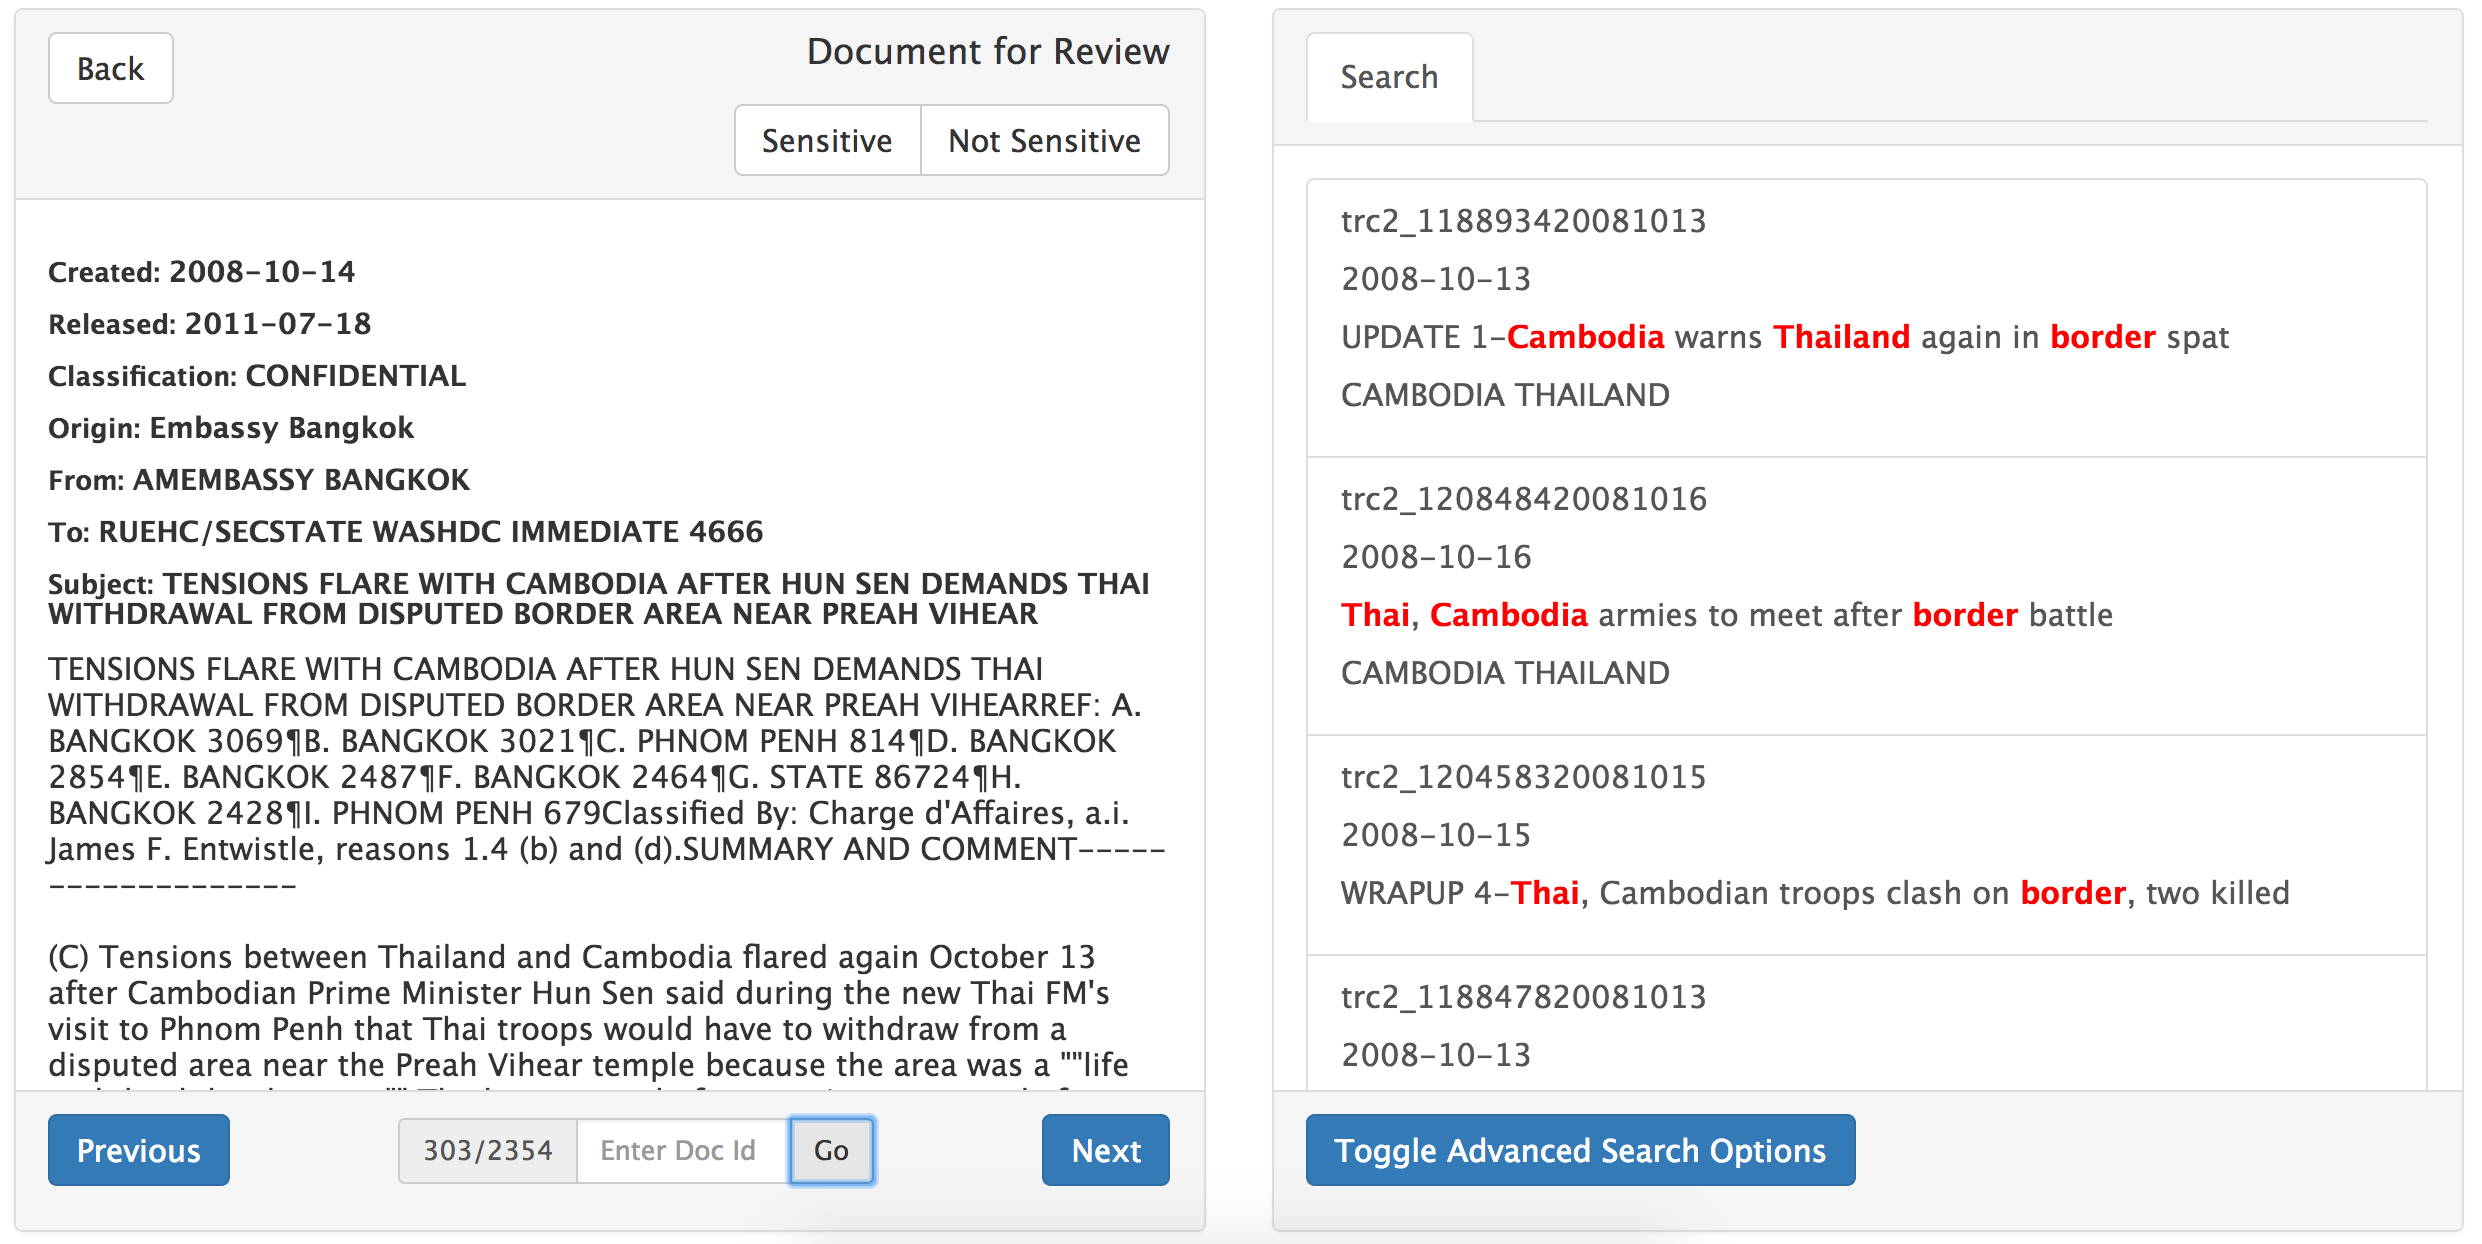
\includegraphics[scale=0.30]{images/searchresults}
\caption{The Front-End Search Results}
\label{relevant_results_full}
\end{figure}
\begin{figure}[H]
\centering
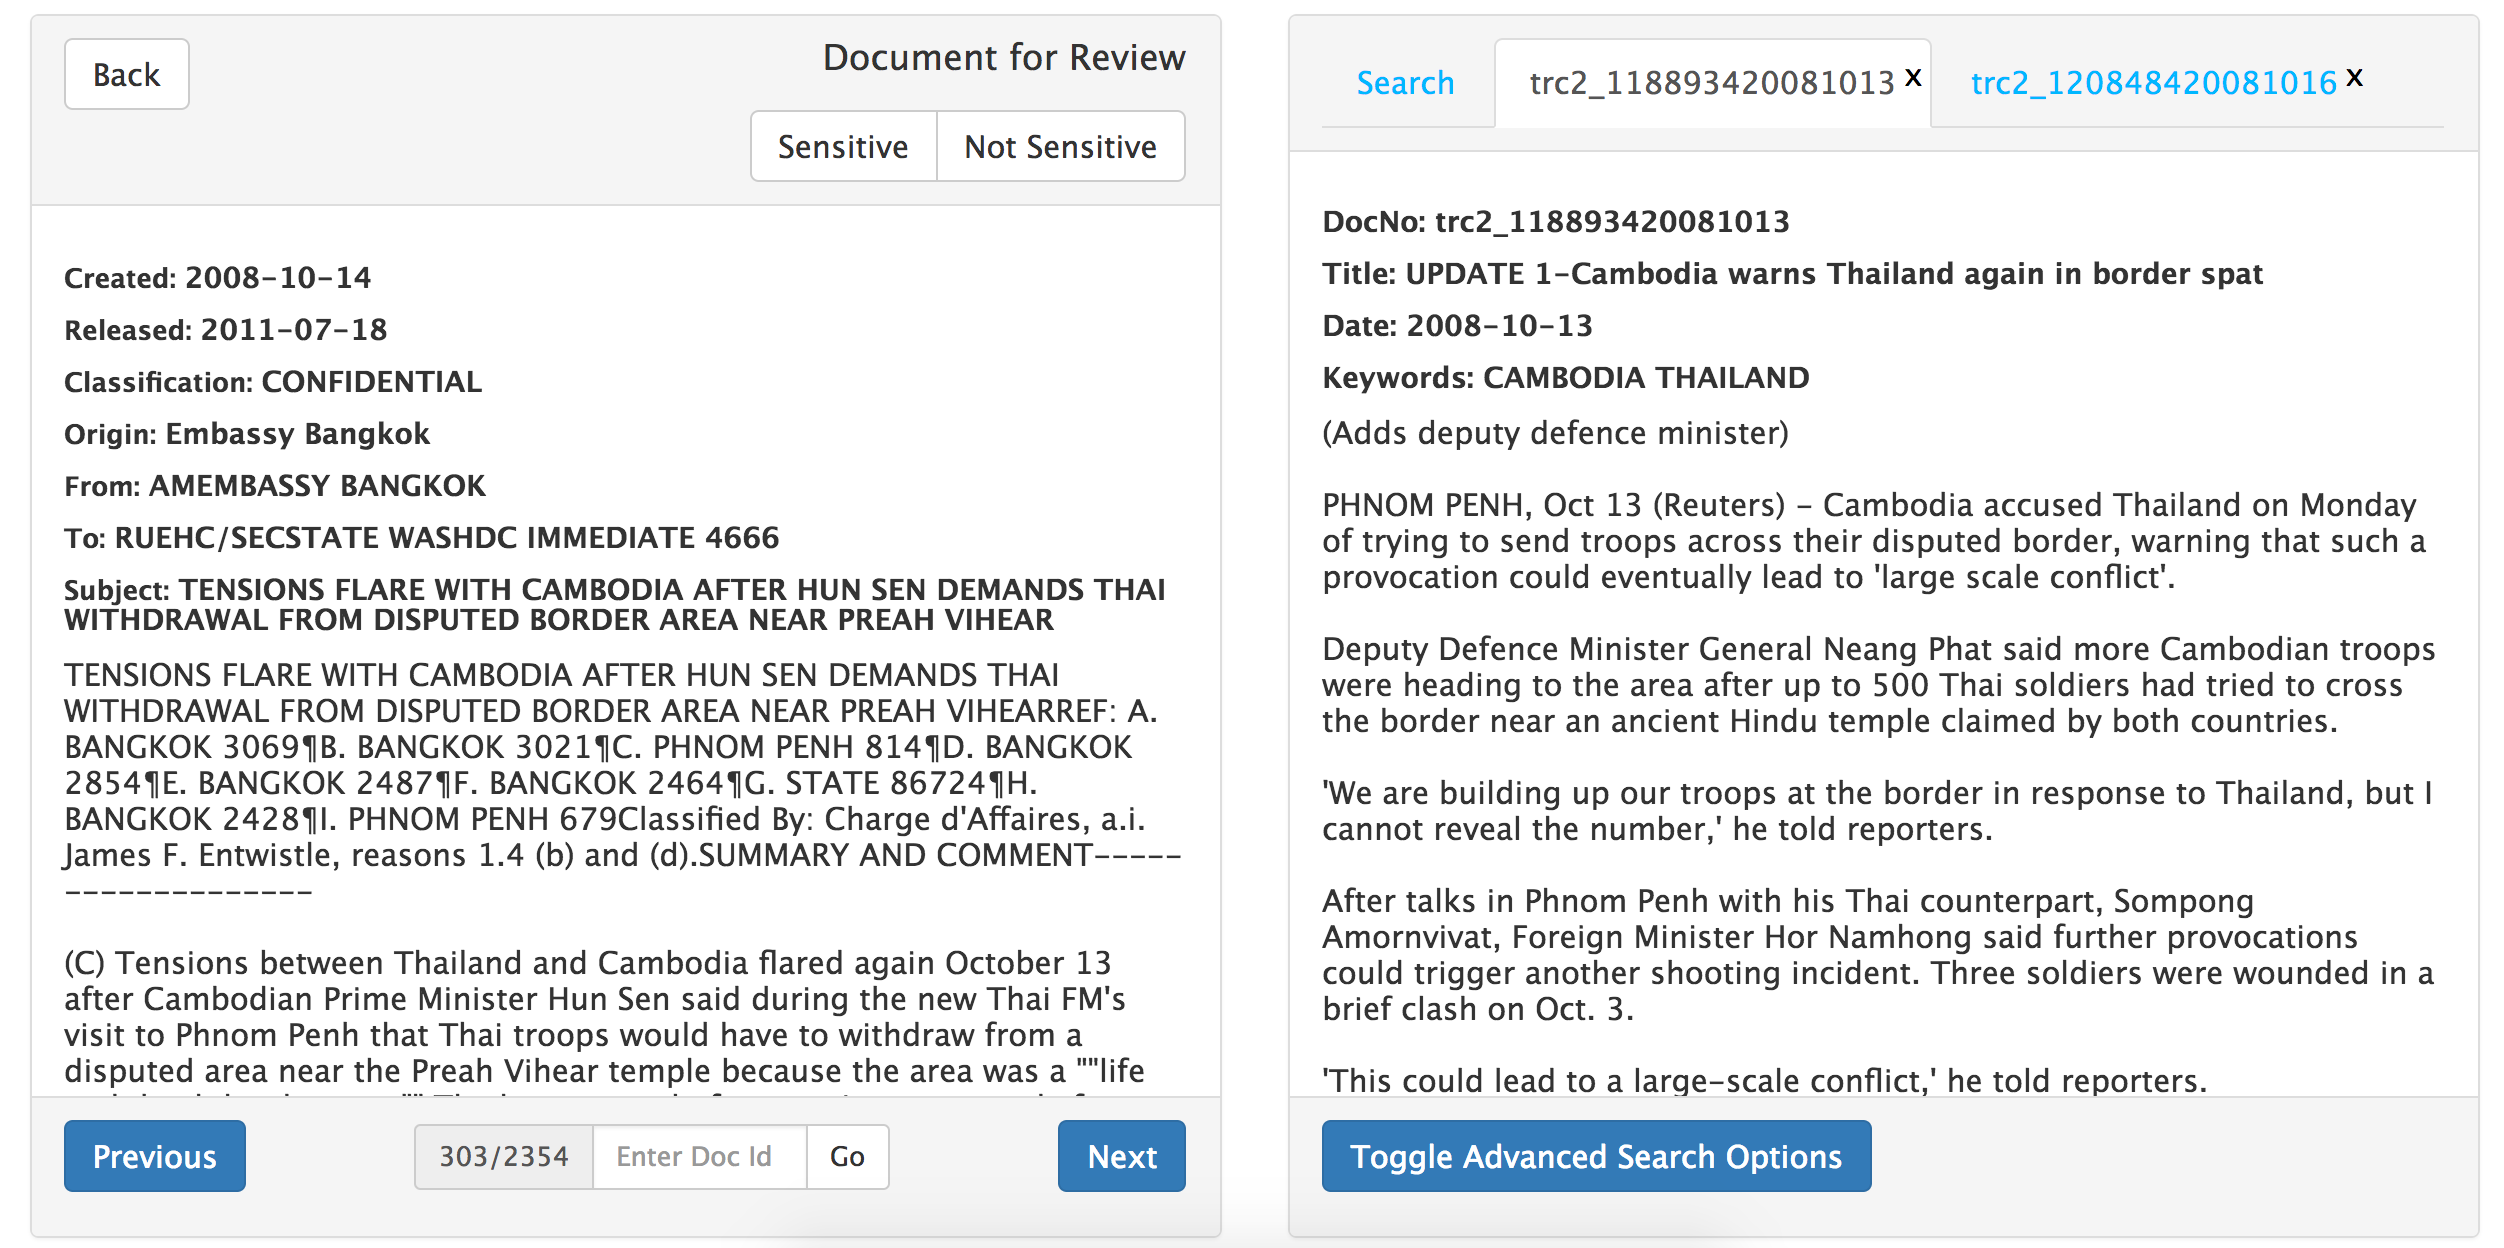
\includegraphics[scale=0.30]{images/targetdocument}
\caption{Viewing a Target Document}
\label{target_doc_view}
\end{figure}

\section{Identifying Sensitivities}
As seen in Figure~\ref{target_doc_view} there are buttons to allow a reviewer to identify a source document as ``Sensitive'' or ``Not Sensitive''. Although not attached to any logic, these serve as a place holder in the prototype for what would eventually be real functionality attached to the document review process. Once out of the prototype stage this project could integrate with current systems that allow documents to be classified. The wording could also be easily changed if necessary. This feature helps to satisfy requirement~\textbf{M.1} by providing a way for a reviewer to identify public domain knowledge in a source document.
\section{Index Choices}
There exists functionality in the frontend to allow a user to choose which index they would like to work on. In a fully functioning system this would be updated to interface with whatever file system or technology is in place.
\section{Summary} \label{clientsummary}
The implementation of the client component of the system did not pose many major difficulties. The single page application provides a functional user interface to interact with the IR capabilities of the server.
The implementation of the client component prompted the following research questions:
\begin{center}
\begin{enumerate}[label=\textbf{Client.\arabic*}]
\item Is the user interface easy to use?
\item Are the documents presented in an intuitive way?
\end{enumerate}
\end{center}

% MAX 8 PAGES
\chapter{Evaluation} \label{evaluation}
This chapter discusses the various stages of evaluation and experimentation performed on the system in an attempt to answer the research questions proposed above and to ensure requirements are fulfilled.
Section~\ref{testing} looks at unit testing to ensure the system is robust, fulfilling~\textbf{NF.5}.
Section~\ref{qualitativeanalysis} refers to some qualitative evaluation and impressions about the system, understood through experimentation and general use.
Section~\ref{offlineevaluation} discusses experiments performed to fulfil \textbf{M.3} and to choose the best query to perform automatically, satisfying \textbf{M.2} and answering research question~\textbf{Server.2}. This section also generally covers how effective query generation was, answering~\textbf{Server.1}
Finally, in Section~\ref{userevaluation} evaluations are conducted in order to look into the thoughts of a potential user of the system and to understand how the UI can be improved for usability to better satisfy~\textbf{NF.1} and answer \textbf{Client.1}~\&~\textbf{Client.2}. 

\section{Testing} \label{testing}
\subsection{Unit Testing}
To ensure \textbf{NF.5} (robustness) was fulfilled, the server component of the system was unit tested. JUnit was used to organise and run unit tests on the various Java classes that comprised this component~\cite{junit}.
The Arrange-Act-Assert pattern was used to organise unit tests in a structured way~\cite{grigg2012arrange}. This allows for clear identification of the method being tested, separate from the code needed to prepare for the test.

Testing necessitated the refactoring of some of the classes which read and write information to files. Many of these classes originally had constructors which took file paths as arguments. The classes would then open the files and read or write to them as necessary.
This approach is inflexible and leads to high coupling~\cite{storer_lecture_2014}. It also means that unit tests need either a sandbox file system to prepare tests, or some kind of mocking of the file system. Mocking a file system is overly complex and adding a sandbox filesystem adds unpredictable side effects.
\begin{codelisting}
\begin{minted}{java}
  // Arrange
  StringReader sr = new StringReader("<DOC>\n"
    + "<DOCNO>docNo value</DOCNO>\n"
    + "<KEYWORDS>keywords value</KEYWORDS>\n"
    + "</DOC>");
  // Act
  TargetDocument doc = new TargetDocument(sr);
  // Assert
  assertEquals(doc.docNo, "docNo value");
  assertEquals(doc.keywords, "keywords value");
\end{minted}
\captionof{listing}{A Unit Test Demonstrating \textit{Arrange, Act, Assert} and a \code{StringReader} Mimicking a File}
\label{code:unittest}
\end{codelisting}
A better, more general, and self contained approach is to have the constructor take a \code{Reader} or \code{Writer} interface as an argument. Any implementing class of these interfaces can then be given as argument to be acted upon for the rest of the operations. This meant that \code{StringReaders} or \code{StringWriters} could be used in unit tests to substitute for real files as seen in Code Sample~\ref{code:unittest}. This approach was extended to several classes which handle interacting with files.

Code which interacted with the Terrier API posed problems in term of unit testing. Terrier often introduces side effects in the form of interacting with established index files in the file system.

The client component of the system was not unit tested, as the logic necessary for its functions was not overly complex. Time constraints necessitated time be spent developing more features. Future work would aim to see a much more robust, tested client application to ensure good usability.

\section{Qualitative Analysis and Defining Relevance} \label{qualitativeanalysis}
Through the course of developing the system and producing the ground truth necessary for the Offline Evaluation as discussed in the Section \ref{offlineevaluation}, certain nuances of the system became clear.

Named entity analysis is not consistent and often produces unexpected or wrong results. Sometimes entities were missed and often words such as ``and'' or ``the'' were tagged as named entities incorrectly. Combating this, the variations of ``and'' and ``the'' created in the named entity identification process were added to the stopwords file to avoid them appearing in queries and being matched in retrieval.

In order to produce the ground truth it was necessary to define returned target documents as ``relevant'' or ``not relevant''. This was extremely nuanced and relied on the discretion of the reviewer. Figure~\ref{fig:comparingtargetdocs} shows the varied target document results when reviewing a source document regarding border clashes between Thailand and Vietnam.
\begin{figure}[H]
\centering
\begin{subfigure}{.5\textwidth}
  \centering
  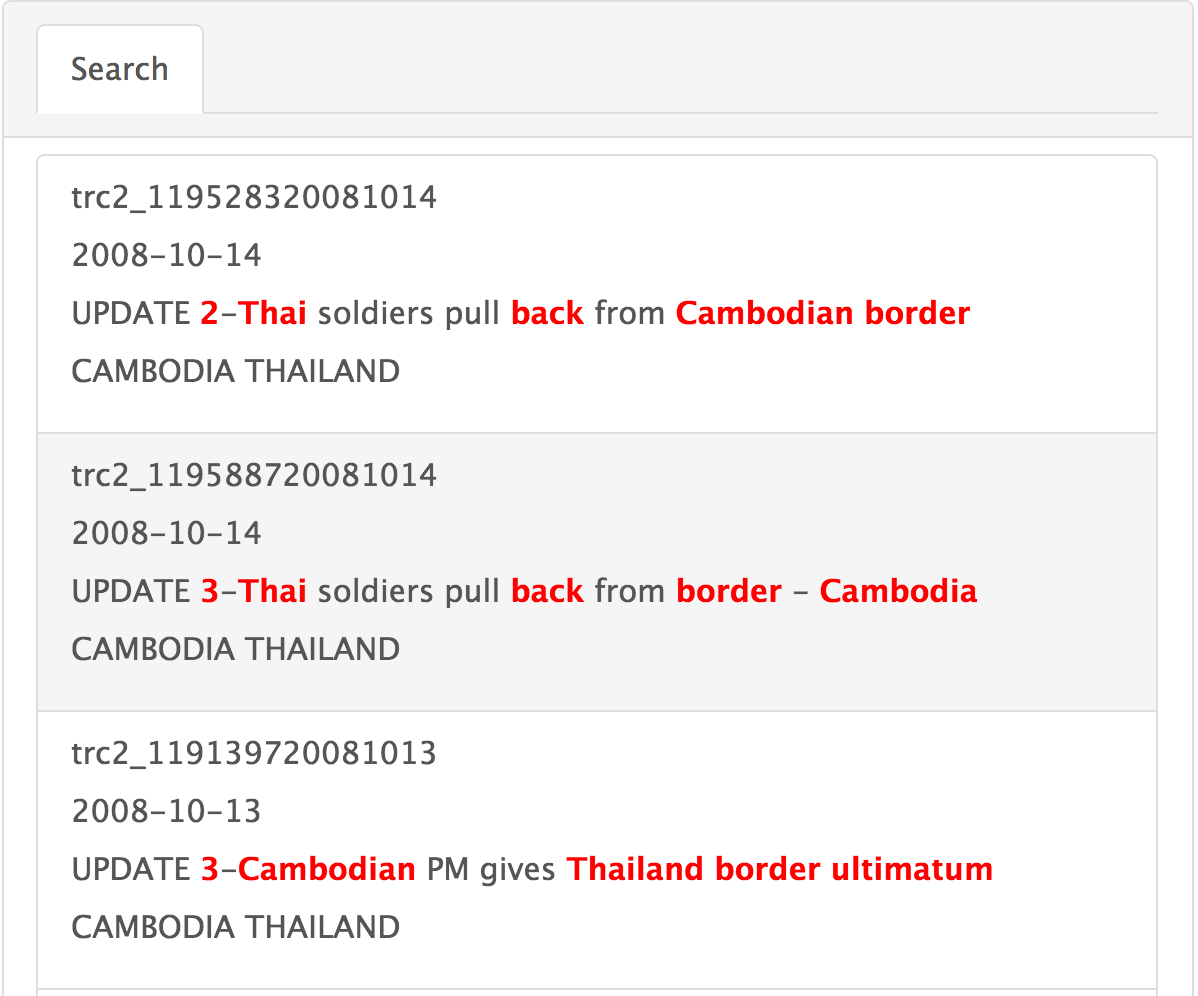
\includegraphics[width=.9\linewidth]{images/good_results}
  \caption{Recognisable Relevant Results}
  \label{relevant_results}
\end{subfigure}%
\begin{subfigure}{.5\textwidth}
  \centering
  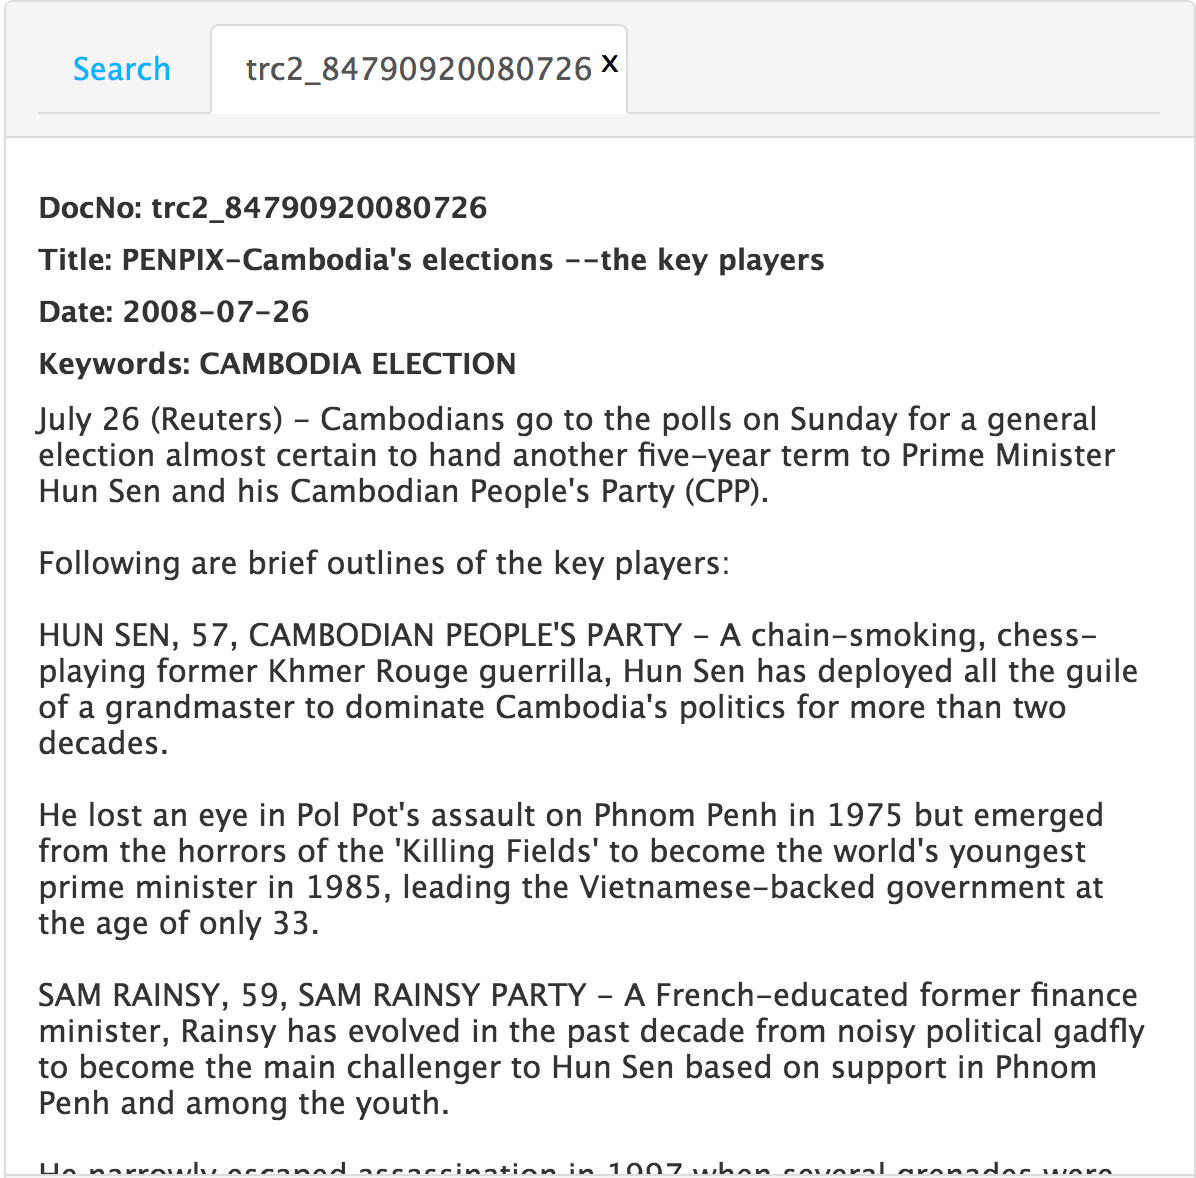
\includegraphics[width=.9\linewidth]{images/bad_result}
  \caption{An Irrelevant Result}
  \label{irrelevant_result}
\end{subfigure}
\caption{Comparing Target Documents}
\label{fig:comparingtargetdocs}
\end{figure}
It is clear why the result shown in Figure~\ref{irrelevant_result} was returned from some formulation of a query, as it mentions Cambodia and their President, however it requires the reviewer to see that it does not mention Thailand or border clashes. Sometimes, this was not as simple and things like dates were important. An example is an article regarding ``Fighting in North Darfur''. The event being referred to was around a specific date, and it had to be ensured that any target document pertaining to fighting in North Darfur matched the correct time frame.

The query formed from Tf-Idf ranking of named entities (see Section~\ref{tfidfquery}) was interesting. It often produced relevant results, but was also the cause of many strange results, such as reports on international sports fixtures. One can see how this occurred, since the names of several countries (often small African nations) not mentioned frequently throughout the collection can push these terms to the top of this query.
In creating the ground truth, it was evident that the system can indeed be used to identify when public domain knowledge exists inside source documents, thereby in part satisfying \textbf{M.1}. It can also be noted that the system performed well when moving through the large collections of source documents and viewing target documents, indicating that it can deal with relatively large amounts of documents, fulfilling \textbf{NF.4} (scalability).

\section{Offline Evaluation Using Terrier}\label{offlineevaluation}
\subsection{Experimental Environment}
Experiments were performed inside a Terrier distribution separate to the main server application. For this experimentation (and throughout development) a collection of source documents analogous to those created by government was used. Target documents consisted of a collection of news articles in the public domain.

For 20 source documents the top 20 results of the 4 query types discussed in Section~\ref{querygen} were marked as either relevant or not relevant. This formed the ground truth or gold standard against which offline evaluations could be run~\cite{Manning:2008:IIR:1394399}. Topics (queries) to be tested exist in \code{.topics} file. These judgements were recorded in a \code{.qrels} file. The system also provided functionality to record the time spent reviewing a target document and a user comment about why the judgement was made. This system could be expanded upon in future work to further understand the document review process.

The offline evaluations were conducted using command line tools provided with Terrier. These can produce customisable and in depth measures of system performance.
One of the most important and relevant measures of IR performance in a system is given by Mean Average Precision (MAP).
MAP is given by:
\begin{displaymath}
  MAP=\frac{\sum_{n=1}^{Q} Ave(P(q))}{Q}
\end{displaymath}
Where: 
\begin{itemize}
\item{~$Q$ is the number of queries.}
\item{~$Ave(P(q))$ is is the average precision of a given query.}
\end{itemize}
\hfill \cite{Manning:2008:IIR:1394399}\\
In order to ensure the choice of query conformed to the non-functional requirements, specifically~\textbf{NF.3} (must return results in reasonable time), mean retrieval time and mean query length are also considered.
\textit{Precision at 1}, \textit{Precision at 4} and \textit{Mean Reciprocal Rank} are also investigated.

It can be assumed Stanford NLP Models with No Distributional Similarity features are used for all experiments other than those in the section which discuss this explicitly (Section~\ref{distsim}).

\subsection{Which Query Formulation is Best?} \label{whichquery}
As posed in the research questions in Section~\ref{serversummary} (specifically, \textbf{Server.2}) it must be investigated which formulation of the query produced from each source document is the most appropriate to be run automatically. The methods used to produce these queries are discussed at length in the Server Implementation chapter, see~\ref{querygen}.
Using the ground truth discussed above Terrier is used to run an offline evaluation with a \code{topics} file consisting of the 4 different query formulations for 20 source documents. These are: \textit{All Terms Query, Named Entities Query, Tf-Idf Named Entities Query,} and \textit{Subject Query}.
\begin{center}
\begin{table}[h]
\centering
\begin{tabular}{|c|c|c|c|c|c|}
\hline
Query					& MAP 				& Mean Query  		& Mean Query 			& Mean Reciprocal 		& Mean Precision 	\\ 
						& 					& Length (Words) 	& Processing Time (s) 	& Rank 					& at 4				\\	\hline
All Terms             	& \textbf{0.4554} 	& 358.5             & 2.51435               & \textbf{0.8500}       & \textbf{0.6750} 	\\	\hline
Named Entities 			& 0.3979 			& 93.45    			& 0.4132 				& 0.7526				& 0.5875 			\\	\hline
Tf-Idf Named Entities 	& 0.3038 			& 10                & \textbf{0.13675}      & 0.7236       			& 0.4375 			\\	\hline
Subject               	& 0.1840 			& \textbf{9.75}     & 0.1578                & 0.3367       			& 0.2500 			\\	\hline
\end{tabular}
\caption{Results of Offline Evaluation}
\label{standard_results}
\end{table}
\end{center}

\begin{figure}[H]
\centering
\begin{subfigure}[t]{.5\textwidth}
\centering
\begin{tikzpicture}
 \begin{axis}[
 	ylabel=$MAP$,
    xlabel={Mean Query Processing Time},
    width=0.95\linewidth,
    height=0.5\linewidth
    ]
        \addplot table[x=time,y=map] {data.csv};
    \end{axis}
\end{tikzpicture}
\end{subfigure}%
~
\begin{subfigure}[t]{.5\textwidth}
\centering
\begin{tikzpicture}
 \begin{axis}[
 	ylabel=$MAP$,
    xlabel={Mean Query Length},
    width=0.95\linewidth,
    height=0.5\linewidth
    ]
        \addplot table[x=length,y=map] {data.csv};
    \end{axis}
\end{tikzpicture}
\end{subfigure}
\caption{Analysis of Mean Average Precision (MAP) Scores against Query Processing Time and Query Length} \label{mapgraphs}
\end{figure}

As seen in Table~\ref{standard_results} and Figure~\ref{mapgraphs}, the All Terms Query consistently performs the best, with little variation, in terms of MAP score. It is however, by far the longest query and so, takes the longest to run. The increase in precision is undoubtedly due to the context provided by including terms which are not themselves named entities.

The \textit{Named Entities Query} performs slightly less well than the \textit{All Terms Query}. It is, however, far faster than the \textit{All Terms Query} as it consists of far fewer terms.

The \textit{Tf-Idf Named Entities Query} performs worse than the \textit{Named Entities Query}. It seems that by eliminating the terms which occur regularly in the document collection some vital terms are removed which increase the precision of a given query.

The \textit{Subject Query} performs the most poorly. This can be expected, as other than running named entity recognition on the line, no other analysis was done to improve its performance. There is also no guarantee that the subject line will contain keywords which provide vital context to a query.
Take, for example, this subject from a document in the source collection:
\begin{center}``PARLIAMENT'S FALL SESSION: A PREVIEW"\end{center}
No insight is given into which country this refers to and although this is not true for many documents, the results clearly demonstrate that the lack of depth in subject queries can cause under-performance.

Although the \textit{All Terms Query} produced the highest MAP scores, it took upwards of 5x as long to run compared to the \textit{Named Entities Query}. At this point the importance of relative result relevance against time concerns must be considered. Users are only willing to wait so long for results (Google and Microsoft suffer business impacts for 0.5s delays!~\cite{performance}).

Aside from MAP score, other measures can be considered. In general, the frontend displays the top 4 results of any given query after automatic querying. Terrier can return measures of the precision specifically for these top 4 results. As seen in Figure~\ref{standard_results}, the \textit{Tf-Idf Named Entities Query} is close to matching the performance of the \textit{All Terms Query} for the these top 4 results. The \textit{All Terms Query} again performs the best, but this can be expected.

Another score which is important and relevant is Mean Reciprocal Rank, which is a measure of how close to the top the first relevant result was ranked. The same narrative presents itself here. The \textit{All Terms Query} performs best, with the \textit{Named Entities Query} scoring relatively high also. The difference in these scores is not great enough to neglect the vast difference in querying time.

As such, the most appropriate query to run automatically is that which consists of Named Entities. Choosing this query ensures Non-Functional Requirements \textbf{NF.2} (relevance) \& \textbf{NF.3} (speed) are fulfilled, as well as ensuring the system is usably fast, answering research question~\textbf{Server.4}.

\subsection{Do StanfordNLP NE Models Affect Search Results?} \label{distsim}
As discussed in Section \ref{classifiers} the named entity identification facility in Stanford NLP can be altered by changing the model used to analyse the text. The same experiment as in Section~\ref{whichquery} is now performed, however this time the Distributional Similarity (Dist-Sim) models are used, which produces remarkably different results, which can be seen in Table~\ref{distsimresults}. This allows us to explore research question \textbf{Server.3}.
\begin{table}[H]
\centering
\begin{tabular}{|c|c|c|c|c|c|}
\hline
Query					& MAP    			& Mean Query		& Mean Query  			& Mean Reciprocal 		& Mean Precision	\\ 
						& 					& Length (Words) 	& Processing Time (s)	& Rank 					& at 4				\\ \hline
All Terms             	& \textbf{0.4397} 	& 337.25            & 2.6132  				& \textbf{0.8750} 		& \textbf{0.6625}   \\ \hline
Named Entities       	& 0.2632 			& 38.8             	& 0.2323    			& 0.6819 				& 0.4625           	\\ \hline
Tf-Idf Named Entities 	& 0.2249 			& 10                & \textbf{0.1506}   	& 0.5857 				& 0.3625        	\\ \hline
Subject               	& 0.2349 			& \textbf{9.75}     & 0.1741   				& 0.5992 				& 0.3250           	\\ \hline
\end{tabular}
\caption{MAP Scores and Query Metrics with Dist-Sim Models}
\label{distsimresults}
\end{table}
\begin{figure}[H]
\centering
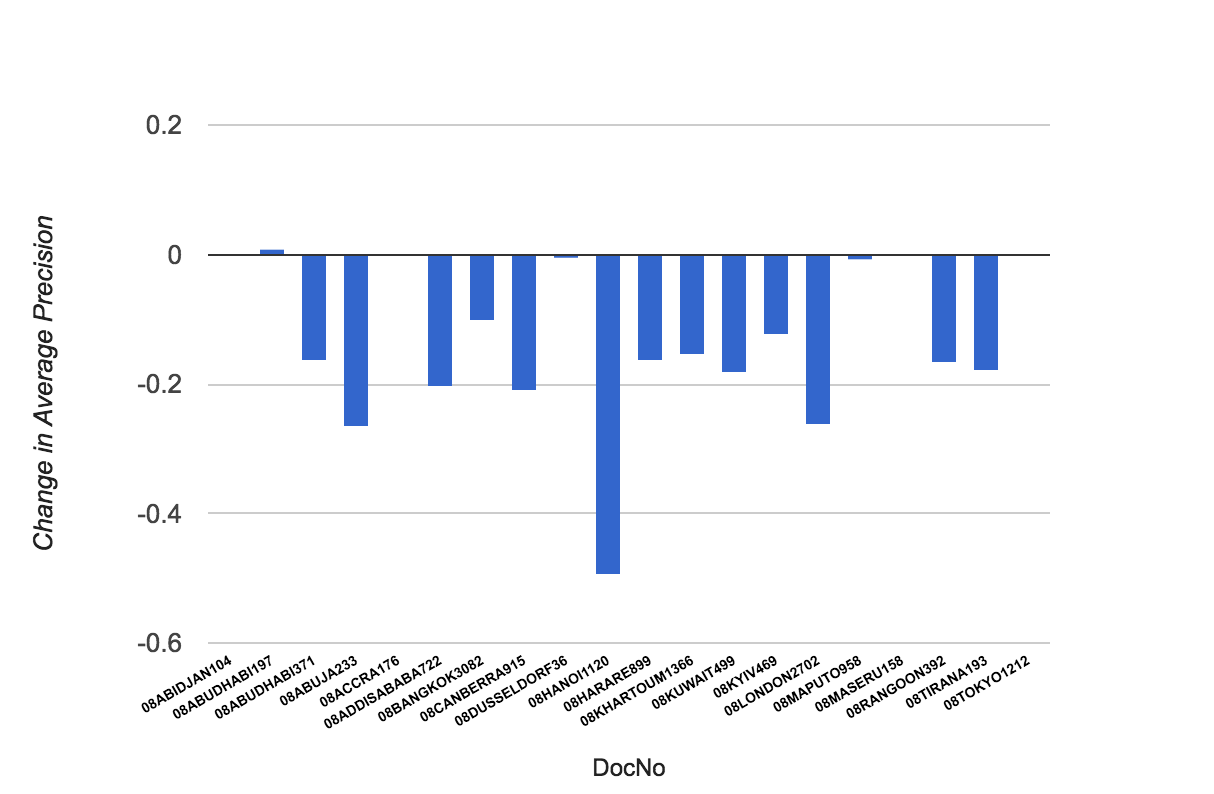
\includegraphics[scale=0.85]{images/query_by_query_change}
\caption{Change in Average Precision When Using DistSim NE Models}
\label{query_by_query}
\end{figure}
It can be seen that, when using the Dist-Sim models, the \textit{All Terms Query} performance did not change by much, however the \textit{Named Entities Query} suffered a large loss in precision. The \textit{Tf-Idf Named Entities Query} was less precise and the \textit{Subject Query} slightly more precise.
Terrier provides the functionality to review evaluation scores on a query by query basis. In Figure~\ref{query_by_query} this is used to show the difference in precision when using the Dist-Sim models compared to the standard no Dist-Sim models. These results are from the \textit{Named Entity Query} in both instances, as this has been identified as the ``best'' query in Section~\ref{whichquery}.

Document~\code{08HANOI1120} exhibits a significant loss in average precision. The \textit{Named Entities Queries} formed when using both types of models can be seen in Appendix~\ref{appendix:hanoiqueries}.
The new query is much shorter, at 33 terms rather than 84 terms. The original (no Dist-Sim Models) query contains terms like `what\_person'', ``security\_person'' and ``end\_location''. These are clearly not named entities and should not be tagged as such. The new (Dist-Sim Models) query seems, upon inspection, to be much more accurate. This example would suggest that the distributional similarity models do, indeed, produce ``better'' named entity tagging. Ironically, this actually worsens the performance of our queries by removing context words that result in better results. This is known to be the case, because these are the type of words that make the \textit{All Terms Query} perform better (as discussed in Section~\ref{qualitativeanalysis}).
These findings indicate that the best precision in the system actually relies on a combination of named entities and other terms. Consequently, it was decided that the No Distributional Similarity Models should be used for now, as these produce the best results for the \textit{Named Entities Query}.
\subsection{Can the Tf-Idf Query Perform Better?}
The \textit{Named Entities Query} performs better than the \textit{Tf-Idf Query} with only 10 terms. It can now be considered whether the number of terms in the \textit{Tf-Idf Query} can improve the performance of this query formulation. The Tf-Idf Query was therefore generated with 5, 10 and 20 terms in order to compare their precision.
\begin{table}[H]
\centering
\begin{tabular}{|c|c|}
\hline
Query Length 	& Mean Average Precision	\\ 
(Words) 		& (MAP) 					\\ \hline
5             	& 0.2861 					\\ \hline
10        		& 0.2635 					\\ \hline
20 				& \textbf{0.2890} 			\\ \hline
\end{tabular}
\caption{Varying \textit{Tf-Idf Query} Length}
\label{tfidflengthresults}
\end{table}
It can be seen from Figure~\ref{tfidflengthresults} that this does not have particularly helpful or conclusive results. The original choice of 10 terms actually performs the worst, with 20 only narrowly beating 5. It seems then, that the top 5 terms are the most important contributor to the \textit{Tf-Idf Query} in terms of precision.
\subsection{Are Some Named Entity Types More Important Than Others?}
The \textit{Named Entities Query} performs well, but it is important to understand if splitting it down into its component parts can reveal which types of named entities have the greatest effect on results.
\begin{table}[H]
\centering
\begin{tabular}{|c|c|}
\hline
Named Entity Type 	& Mean Average Precision	\\ 
					& (MAP) 					\\ \hline
Person          	& \textbf{0.1236} 					\\ \hline
Location			& 0.1070 					\\ \hline
Organisation 		& 0.0303 					\\ \hline
\end{tabular}
\caption{Querying Using Only 1 Named Entity Type}
\label{namedentityresults}
\end{table}
From Table~\ref{namedentityresults} it appears that the ``person'' named entities have the greatest impact on results. When considering future query formulations emphasis on ``person'' named entities should be increased.
\subsection{What makes a query good or bad?}
The queries formed from source documents \code{08ACCRA176} and \code{08MASERU158} score 0 precision in all four categories. This can be put down to the content of both of these documents. \code{08ACCRA176} describes a meeting of Ghanaian official following the raid of a brothel and \code{08MASERU158} describes a public transportation dispute. These stories are very local and so the number of relevant documents to find in the target collection will be vanishingly slim. \\
\paragraph{Precision at 1 and Reciprocal Rank}
Intuitively, the top result of a query is the most important one, and is the result the reviewer will be most likely to look at. It is important then to consider the ``Precision at 1'' of the queries. This whether or not the top result is relevant for a given query.
Reciprocal rank can also be considered. This is a measure of how close to the highest ranking the first relevant document appears. When considering the \textit{Named Entities Query}, by far the worst performing source document was: \code{08TOKYO1212} (other than \code{08ACCRA176} \& \code{08MASERU158} which are discussed above). This document is addressing the issue of ``cluster munitions'' primarily. This is not a named entity and so will not be included in the \textit{Named Entities Query}. If evaluation results of the corresponding \textit{All Terms Query} are reviewed a near 100\% increase in reciprocal rank can be seen, indicating that the inclusion of more context terms improve results. This reinforces the points made in Sections~\ref{whichquery}~\&~\ref{distsim}.

\section{User Evaluation} \label{userevaluation}
User evaluations are performed to ensure the product is satisfactory to end users. Since this project was an experiment and a prototype, mainly focussing on IR techniques, it was less important to rigorously evaluate the frontend.
\subsection{Think-Aloud}
Timothy Gollins, Head of Digital Archiving at the National Records of Scotland, and key potential beneficiary of this project participated in a think-aloud study while examining the software in use. Also being former Head of Digital Preservation at The National Archives (UK), Timothy has expert insight into the problem domain.
Some of the key points learned from this session are listed below:
\begin{itemize}
\item \textit{``Named Entity importance is nuanced and frequency (or Tf-Idf) of named entities does not necessarily produce the most important terms.''}
\par
This raises an important point regarding the limitations of automatic query generation. The system must allow the user to run custom queries and in the future, explore and learn from how real users formulate their queries. This suggests that the machine learning identified in Requirements \textbf{C.1} could be very useful.
\item \textit{``Further term highlighting or importance weighting is necessary to help produce the best results.''}
\par
This point highlights the fact that the queries generated right now are fairly general, and some deep understanding of the way archivists review documents could help produce better results. Briefly mentioned was weighting the first and last paragraphs higher than the middle of the document, as these are likely to contain the most pertinent information. This again confirms the last point.
\item \textit{``More advanced methods could be leveraged to improve yet further the capabilities of the software, like eye tracking or automatic querying upon clicking terms.''}
\par
Although beyond the scope of this project, this point identifies the potential expansion of this project. Eye-tracking could be used to automatically track what the user is interested in from the source document, forming the basis of new automatic queries. A simplified version of this could use clicking to accomplish the same results.
\item \textit{``UI considerations are equally as important as information retrieval considerations when it comes to improving the effectiveness of the software.''}
\par
At this point in the project, the implementation of most of the IR functionality was complete. It now became important to consider how best to modify and improve the user interface to ensure the easiest experience possible. It was at this point, and in direct reaction to this comment, that decoration was implemented (see Sections~\ref{client_decoration}~\&~\ref{server_decoration}).
\end{itemize}
Further to the above points, the participant was generally very enthusiastic about the applications of such a system and made it clear that this would be an extremely welcome introduction to the problem of sensitivity review. The user interface was clear and unambiguous and allowed discussing of the more specific points above.
This user evaluation helps to answer the research questions about usability from Section~\ref{clientsummary}. It also addresses Non-Functional Requirement \textbf{NF.1}, in that the system is somewhat intuitive, but improvements could be made.
The system needs to do everything possible to highlight potential matches between source and target documents in order to help the reviewer identify public domain knowledge in the most efficient way.

\section{Summary}
Primarily the evaluations addressed the research questions proposed in Sections~\ref{serversummary}~\&~\ref{clientsummary}.
Answering \textbf{Server.1}, query generation is somewhat effective, however could be improved through greater research and understanding. The \textit{Named Entities Query} was found to be ``best'', as it produced relatively good results within reasonable time. This answers \textbf{Server.2}. In investigating \textbf{Server.4} it can be seen that the StanfordNLP models have a considerable effect on the performance of queries and that with added analysis, this could be optimised. The system is usably fast, answering \textbf{Server.4}, although only because the query choice is in line with this concern. As for the concerns of \textbf{Client.1}~\&~\textbf{Client.2} the user interface is fairly easy and intuitive to use, as exemplified through a think aloud. It could be improved somewhat, however provides an excellent starting point for future work.

These evaluations drove changes to improve the project in various ways. The most appropriate query to automatically run was chosen and the best means (currently) of identifying named entities was identified. The IR accuracy was further increased by altering the stopwords file to remove incorrect named entities and terms. User evaluation drove the implementation of decoration to ensure the frontend was as intuitive as currently possible.

There are, however, many more changes that could be made to improve the performance of the system that were infeasible to implement within the time frame of the project.
More decoration could be applied to target documents when displayed in full to help reviewers more easily spot similarities.
Named entity recognition could be continually refined to ensure the best queries possible are formed. This could even come in the form of multiple indexes against which to run different queries, with each using different named entities techniques.
The evaluations highlighted the successes and shortcomings of the project, answered the research questions proposed during implementation and ensured the requirements were fulfilled.

% MAX 2 PAGES
\chapter{Conclusions} \label{conclusion}
\section{Fulfilled Requirements}
The Identifying Public Domain Knowledge project set out to create a system capable of improving the document review system necessary as digital records become more and more widespread.
The final product satisfies all of the Must Have requirements and addresses some of the Should and Could Have sections. In terms of these requirements, the project can be classified as a success. More generally the project certainly addresses the needs set out in Section~\ref{needs}. The tool is fairly efficient and effective for reviewing documents addressing \textbf{Need.1}. \textbf{Need.2} is satisfied through automatic querying for target documents and the two panel display interface. \textbf{Need.3} is addressed by the tool not accessing information on the internet. All information is stored locally on the server, preventing sensitive searches from being exposed.

It demonstrates the applications IR and technology can have in the field of sensitivity review and paves the way for continued work to improve the ability of government to be transparent and fair, a matter which is very relevant in today's geo-political landscape. The project fails, however, to deal with all of the requirements and lacks some features which could greatly improve the usability and functionality.

\section{Opportunities for Future Work}
If work were to continue on this project many sections could be improved and new features could be introduced. Addressing the concerns raised in Chapter~\ref{evaluation} it would be highly advisable to experiment more thoroughly with different query formulations to achieve the very best performance possible. This would require lots of very domain specific tweaking and testing. A key initial improvement may be to implement date analysis to ensure target documents are with in a reasonable time frame. This was identified as requirement~\textbf{S.3} but was never implemented due to time constraints.
Further to this, it would be achievable and worthwhile to perform better key phrase extraction upon source documents to form queries with named entities and context, other than the behemoth \textit{All Terms Queries} which took too long to return results.

Further in the future, machine learning could be introduced into the system so it could begin to improve over time and with repeated use. This would be more useful if the product could be used in a real working environment, so it could adapt to the procedures of its end users.
Even later in development, improved HCI features like eye tracking could be implemented to truly respond in real time to user input, but this would require all other aspects of the system to be much more robust.

\section{Reflection}
As a developer, I learned many things during the course of this project. Some of these things were technical, like a new found understanding of IR concepts and REST API design. However much of what was learned was regarding the effective planning and execution of a long term solo-project. Early planning and research is vital and I feel that could I repeat the project I would have made efforts to organise the early stages of development far better. This led to some negative impacts towards the end of the project, resulting in some features not being implemented (like date range searching). I am, however, very happy with the work I did complete and I have a keen interest in continuing research in the fields of IR and Sensitivity Review.

%%%%%%%%%%%%%%%%
%              %
%  APPENDICES  %
%              %
%%%%%%%%%%%%%%%%
\begin{appendices}
\chapter{Examples of Queries}
\begin{codelisting}
\begin{minted}[breaklines,breaksymbolleft={}]{xml}
s countries lrb  state_location who  rrb   will 24 participate made tell event 30 told attending  give suggested demarche iran_location added officer ref foreign_organization department_organization likely formal  nuclear group_organization reasons conference comments attend uk_location political_organization office_organization regional_organization discourage coordination_organization activities poloff_person claims classified 14 c_organization london_location points separately conference_organization mills_person leader consistent ngos_organization team_organization october_person contacts nuclear_organization website november_organization advisable intend substance will_person attendance iran_organization credibility visit_location hmg_organization counselor_organization academics will_location commonwealth_organization xxxxxxxxxxxx_person conference_location nuclear_location 112229 rick_person craig_person amenable rachel_person nonattendance fco_organization tuttle participate_organization martinek_person lesley_person counterproliferation_organization
\end{minted}
\captionof{figure}{An Example All Terms Query}
\label{code:all_terms_query}
\end{codelisting}
\begin{codelisting}
\begin{minted}[breaklines,breaksymbolleft={}]{xml}
state_location iran_location foreign_organization department_organization group_organization uk_location political_organization office_organization regional_organization coordination_organization poloff_person c_organization london_location conference_organization mills_person ngos_organization team_organization october_person nuclear_organization november_organization will_person iran_organization visit_location hmg_organization counselor_organization will_location commonwealth_organization xxxxxxxxxxxx_person conference_location nuclear_location rick_person craig_person rachel_person fco_organization participate_organization martinek_person lesley_person counterproliferation_organization
\end{minted}
\captionof{figure}{An Example Named Entities Query}
\label{code:ne_query}
\end{codelisting}
\begin{codelisting}
\begin{minted}[breaklines,breaksymbolleft={}]{xml}
craig_person fco_organization hmg_organization participate_organization martinek_person lesley_person counterproliferation_organization iran_location rachel_person rick_person
\end{minted}
\captionof{figure}{An Example TF-IDF Named Entities Query}
\label{code:tf_idf_query}
\end{codelisting}
\pagebreak
\begin{codelisting}
\begin{minted}[breaklines,breaksymbolleft={}]{xml}
uk will not participate in irans_location nuclear conference will discourage others from attending ref state 112229
\end{minted}
\captionof{figure}{An Example Subject Query}
\label{code:subject_query}
\end{codelisting}
\chapter{Named Entity Queries for \code{08HANOI1120}} \label{appendix:hanoiqueries}
\begin{codelisting}
\begin{minted}[breaklines,breaksymbolleft={}]{xml}
council_organization summary_location sbu_organization comment_organization ambassador_location us_location united_location control_organization embassy_organization states_location affairs_organization end_location end_organization office_organization government_organization committee_organization department_organization state_organization land_location ministry_organization c_organization security_organization foreign_organization on_organization social_organization but_organization chairman_organization public_organization alike_person s_organization allow_location media_location people_organization vietnam_location what_person outreach_organization catholic_organization continued_location freedom_person freedom_organization demonstrations_organization church_organization catholics_person thai_location hanoi_organization gvn_organization hanoi_location vietnamese_location hanoi_person dung_person religious_person thai_organization parish_location ha_location quang_person religious_organization ngo_person church_location papal_organization archbishop_organization kiet_person parishioners_organization joseph_person archbishop_person papal_location nunciate_organization nuncio_location ap_organization papal_person nuncio_person county_location speculating_person irf_organization pope_person orange_location disputes_location papul_location vatican_location vatican_organization religious_location karaoke_person vexed_organization septebmer_organization ha_organization
\end{minted}
\captionof{figure}{Named Entity Query When Using Models Without Distributional Similarity}
\label{code:hanoiwithout}
\end{codelisting}
\begin{codelisting}
\begin{minted}[breaklines,breaksymbolleft={}]{xml}
council_organization sbu_organization us_organization us_location united_location states_location affairs_organization office_organization ministry_organization on_organization government_organization foreign_organization committee_organization s_organization embassy_organization security_organization vietnam_location people_organization catholic_organization public_organization church_organization hanoi_location quang_person ngo_person kiet_person joseph_person hanoi_organization religious_organization county_location orange_location archbishop_person vatican_location vatican_organization
\end{minted}
\captionof{figure}{Named Entity Query When Using Models With Distributional Similarity}
\label{code:hanoiwith}
\end{codelisting}

\begin{figure}[t]
\centering
\begin{tikzpicture}
 \begin{axis}[
 	ylabel=$MAP$,
    xlabel={Mean Query Processing Time},
    width=0.50\linewidth,
    height=0.25\linewidth
    ]
        \addplot table[x=time,y=map] {data.csv};
    \end{axis}
\end{tikzpicture}
\end{figure}

\end{appendices}

%%%%%%%%%%%%%%%%%%%%
%   BIBLIOGRAPHY   %
%%%%%%%%%%%%%%%%%%%%

\bibliographystyle{plain}
\bibliography{bib}

\end{document}
